\documentclass{book}
\usepackage{geometry}
\usepackage[utf8]{inputenc} % UTF-8 unterstützung
\geometry{papersize={170mm,240mm},total={140mm,200mm},top=21mm,bindingoffset=10mm}
\usepackage{ngerman}
\usepackage{times}
\usepackage{amsmath}
\usepackage{amssymb}
\usepackage{amsfonts}
\usepackage{amsthm}
\usepackage{graphicx}
\usepackage{fancyhdr}
\usepackage{textcomp}
\usepackage[all]{xy}
\usepackage{txfonts}
\usepackage{alltt}
\usepackage{verbatim}
\usepackage{paralist}
\usepackage{makeidx}
\usepackage{array}
\usepackage{hyperref}
\usepackage{xcolor}
\usepackage{listings}
\lstdefinestyle{Matlab}{
  numbers=left,
  belowcaptionskip=1\baselineskip,
  breaklines=true,
  frame=L,
  xleftmargin=\parindent,
  language=Matlab,
  showstringspaces=false,
  basicstyle=\footnotesize\ttfamily,
  keywordstyle=\bfseries\color{green!40!black},
  commentstyle=\itshape\color{purple!40!black},
  identifierstyle=\color{blue},
  stringstyle=\color{orange},
  numberstyle=\ttfamily\tiny
}
\lstdefinestyle{C}{
  numbers=left,
  belowcaptionskip=1\baselineskip,
  breaklines=true,
  frame=L,
  xleftmargin=\parindent,
  language=C,
  showstringspaces=false,
  basicstyle=\footnotesize\ttfamily,
  keywordstyle=\bfseries\color{green!40!black},
  commentstyle=\itshape\color{purple!40!black},
  identifierstyle=\color{blue},
  stringstyle=\color{orange},
  numberstyle=\ttfamily\tiny
}
\usepackage{caption}
\usepackage{subcaption}
\usepackage{epstopdf}
\usepackage{standalone}
\usepackage[backend=bibtex]{biblatex}
\addbibresource{MonteCarlo.bib}



\begin{document}
\title{Monte Carlo Methode}
\author{Dorian Amiet, Hannes Badertscher}
\date{}
\maketitle



\chapter{Die Monte Carlo Methode}
\rhead{Die Monte Carlo Methode}
\begin{refsection}

\section{Einleitung}
Der Monte Carlo Algorithmus ist ein Verfahren zur Lösung numerischer Probleme durch das Ziehen von Zufallszahlen. Die Idee, mathematische bzw. physikalische Probleme mit einem stochastischen Sampling-Verfahren zu approximieren stammt polnisch-amerikanischen Mathematiker Stanisław Marcin Ulam (1909 -- 1984), welcher zu dieser Zeit im Los Alamos National Labaratory arbeitete. Seine Idee, und wie es dazu kam, beschrieb er folgendermassen: \\

\begin{quote}
\textit{“The first thoughts and attempts I made to practice [the Monte Carlo method] were suggested by a question which occurred to me in 1946 as I was convalescing from an illness and play- ing solitaires. The question was what are the chances that a Canfield solitaire laid out with 52 cards will come out successfully? After spending a lot of time trying to estimate them by pure combinatorial calculations, I wondered whether a more practical method than “abstract thinking” might not be to lay it out say one hundred times and simply observe and count the number of successful plays. This was already possible to envisage with the begin- ning of the new era of fast computers, and I immediately thought of problems of neutron diffusion and other questions of mathematical physics, and more generally how to change processes described by certain differential equations into an equivalent form interpretable as a succession of random operations. Later... [in 1946, I ] described the idea to John von Neumann and we began to plan actual calculations.”} - Stan Ulam, 1983
\end{quote}

Als erste Anwendung konnten Ulam und von Neumann mit der Monte Carlo Methode die Neutronen-Diffusion in spaltbaren Materialien simulieren. 

\subsection{Anwendungen}

Monte Carlo Methoden kommen überall zum Einsatz, wenn deterministische Algorithmen entweder zu komplex sind, oder gar nicht existieren. Dank zunehmender Rechenleistung sind in den letzten Jahren Simulationen wie globale Klimamodelle möglich geworden. Typische Anwendungen des Monte Carlo Algorithmus umfassen u.a.

\begin{itemize}
	\item Numerische Integration
	\item Simulation von dynamischen Prozessen
	\item Simulation von Gleichgewichtszuständen (z.B. mit Metropolis-Algorithmus)
	\item Statistische Untersuchung von Zufallsverteilungen
\end{itemize}


\section{Zufallszahlengeneratoren}

\begin{quote}
\textit{“Anyone who considers arithmetical methods of producing random digits is, of course, in a state of sin.”} - John von Neumann, 1951
\end{quote}

Die Generierung von Zufallszahlen ist absolut essentiell für die Monte Carlo Methode. In der analogen Welt bestehen verschiedene hervorragende Zufallsgeneratoren, u.a. das thermische Widerstandsrauschen oder radioaktive Zerfallsvorgänge. So gab es in der Vergangenheit Ansätze, in welchen die Strahlung einer radioaktiven Quelle gemessen wurde und daraus eine Folge von Zufallszahlen generiert wurde. Heute werden eher Rauschgeneratoren mit Widerständen oder Dioden verwendet. In digitalen Schaltungen wird teilweise der Ausgang eines metastabilen Flip-Flop als Zufallszahlengenerator verwendet.\\

In Software ist es deutlich schwieriger, ``gute'' Random Number Generators (RNGs) zu realisieren. Technisch gesehen sind Software RNGs immer \textit{Pseudo} Random Number Generators (pRNGs),  denn der Ausgangswert eines deterministischen Programms kann per Definition nicht zufällig sein. Die Schwierigkeit ist es, Zahlen zu generieren, die aus der Perspektive des Anwenders komplett zufällig sind, obwohl sie eindeutig mathematisch definiert sind.

\newpage
\subsection{Random-Device} \label{subsec:RandomDev}

Auf Unix-Systemen steht mit dem sog. Random-Device (/dev/random) ein Zufallszahlengenerator sehr hoher Güte zur Verfügung. Dieser sammelt das Rauschen von Gerätetreibern in einem Entropie-Pool und generiert daraus Zufallszahlen, welche auch höchsten Anforderungen im Bereich der Kryptografie genügen. Der Nachteil ist, dass sobald dieser Entropie-Pool erschöpft ist keine Zufallszahlen mehr generiert werden können. Mit dem Device /dev/urandom wurde Abhilfe geschaffen, was jedoch mit dem Nachteil erkauft wird, dass beim Unterschreiten einer gewissen Entropie-Schwelle nur Pseudozufallszahlen generiert werden, welche unter Umständen von einem potentiellen Angreifer berechnet werden könnten. Den meisten Anforderungen genügt dies jedoch trotzdem. \\

Das Random-Device kann von einem Programm wie ein File eingebunden werden und Zufallszahlen daraus gelesen werden. Für viele Anwendungen ist dies klar zu langsam, weshalb häufig das Random-Device nur als Seed für einen Pseudo-Random-Number-Generator verwendet wird.

Ein Code-Snippet zur Verwendung des Random-Device ist im Github-Repository \cite{rng:githubRepo} zu finden.

Abbildung \ref{fig:dev_rand_histogram} zeigt ein Histogramm von $1'000'000$ Zufallszahlen zwischen $0$ und $1$, welche vom Random-Device eingelesen wurden.

\begin{figure}[htbp]
	\centering
	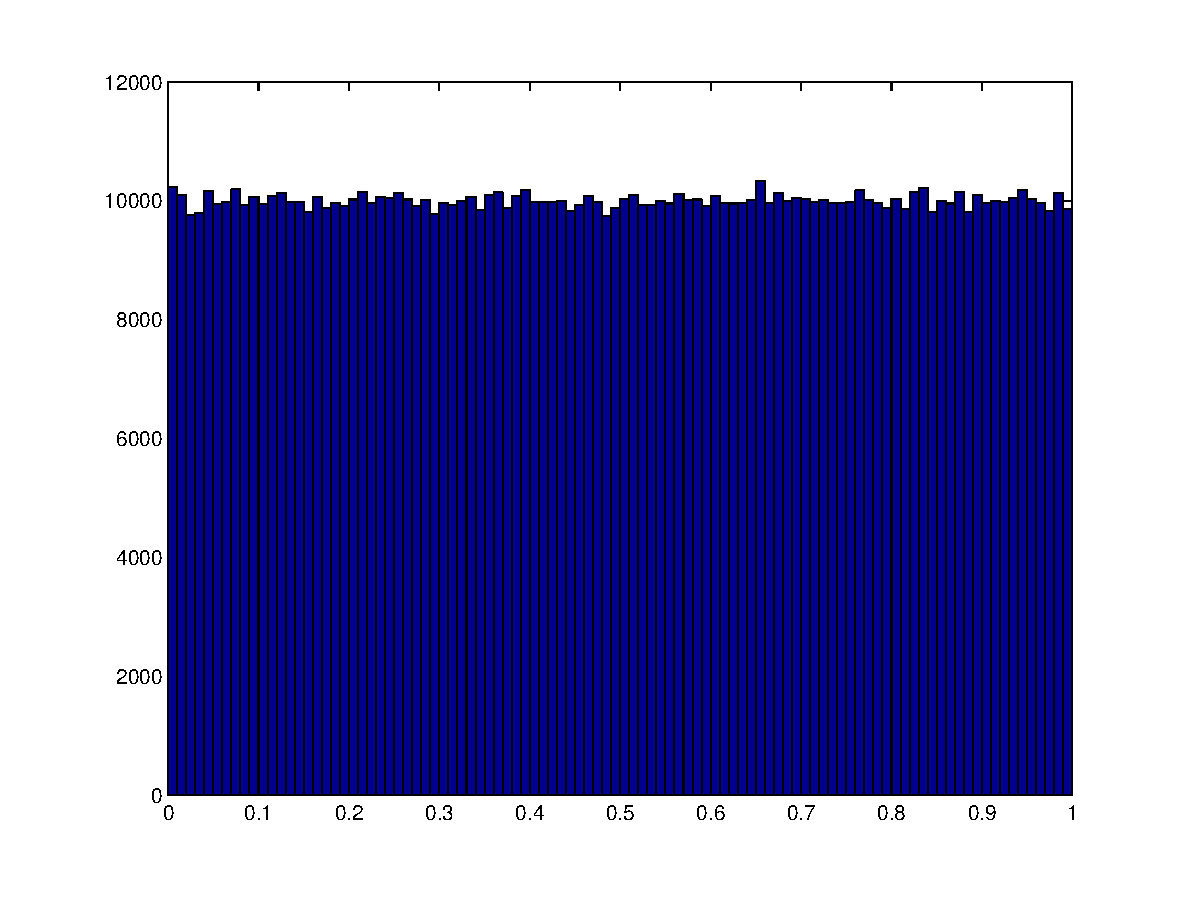
\includegraphics[width=8cm]{images/dev_rand_histogram.eps}
	\caption{Histogramm von $1'000'000$ Zufallzahlen im Interval $[0,1]$ des Random-Device}
	\label{fig:dev_rand_histogram}
\end{figure}

\newpage
\subsection{Multiplikativ kongruentielle Generatoren (LCG)} \label{subsec:LCG}
Eine der populärsten Methoden zur Generierung von Zufallszahlen ist die multiplikativ kongruentielle Methode. Solche Generatoren werden häufig als \textit{linear congruential generator (LCG)} bezeichnet. Dabei werden Zufallszahlen rekursiv nach folgender Vorschrift berechnet:

\begin{equation}
	x_{i+1} = \left( a x_{i} + b \right) \mod{m}
	\label{equ:lcg_equation}
\end{equation}

Der Generator ist durch den Startwert $x_1$, den Faktor $a$, das Inkrement $b$ und das Modul $m$ vollständig bestimmt. Ein LCG generiert Zufallszahlen zwischen $0$ und $m-1$. Für viele Zwecke sind gleichverteilte Zufallszahlen zwischen $0$ und $1$ gefragt. Diese werden wie folgt berechnet:

\begin{align}
	y_i &= \frac{x_i}{m} \: &\text{for approx. uniformly distributed numbers  in } [0,1)\\
	y_i &= \frac{x_i}{m-1} \: &\text{for approx. uniformly distributed numbers in [0,1]}
\end{align} 


LCG Generatoren sind sehr stark von der Wahl der Konstanten $a$,$b$,$m$ abhängig. Eine suboptimale Wahl kann zu einer sehr geringen Periode und einer eindeutigen Korrelation aufeinanderfolgender Zahlen führen. Abbildung \ref{fig:lcg_verteilung} verdeutlicht dies anhand eines LCG mit $a=11$, $b=0$ und $m=64$. \\

\begin{figure}[h]
	\centering
	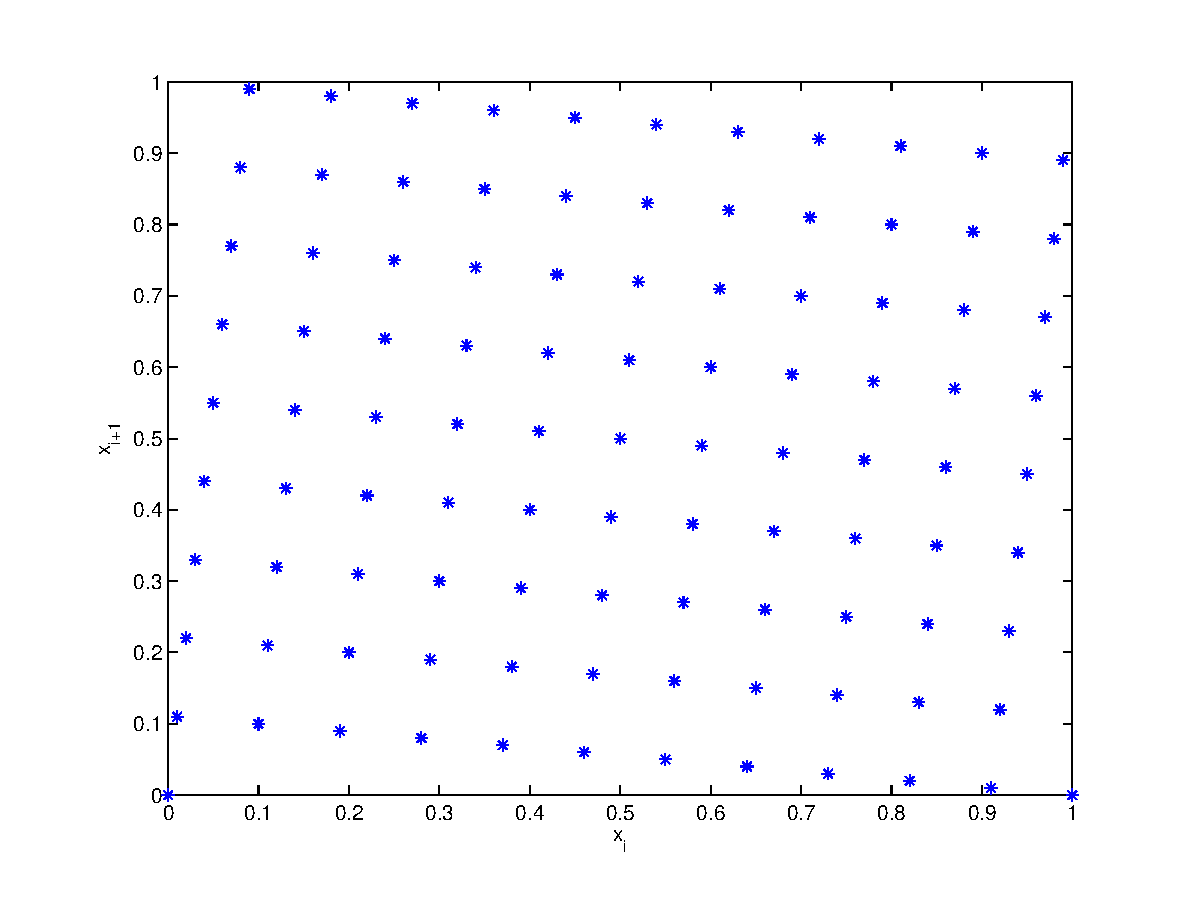
\includegraphics[width=8cm]{images/lcg.eps}
	\caption{Verteilung aufeinanderfolgender Zufallszahlen eines LCG mit $a=11$, $b=0$, $m=64$}
	\label{fig:lcg_verteilung}
\end{figure}

\subsubsection{Die IBM RANDU-Funktion}
Ein bekanntes Beispiel für schlecht entwickelte LCG Generatoren ist die Funktion \textit{RANDU}, welche ab den 60er-Jahren eine Standardfunktion auf dem IBM System/360 war. Diese nutzte einen LCG-Algorithmus gemäss folgender Gleichung:

\begin{equation}
	x_{i+1} = \left( 65539 \: x_i \right) \mod{2^{31}}
	\label{equ:ibm_randu}
\end{equation}

Mit $m = 2^{31}$ reduziert sich die Modulo-Operation in einem 32-bit System auf einen kontrollierten Overflow. Mit $a = 65539 = 2^{16} + 3 = 10\cdots011_{\text{bin}}$ wird die Multiplikation zu Additionen und Bit-Shifts vereinfacht. Der Algorithmus ist damit hocheffizient, hat aber folgendes Problem. \\

Aus der Zuordnungsvorschrift
\begin{equation*}
	x_{i+1} = (2^{16} + 3) x_i
\end{equation*}
folgt für zwei Iterationen:
\begin{align*}
	x_{i+2} &= (2^{16} + 3) x_{i+1} \\
	 &= (2^{16} + 3)^2 x_i \\
	 &= [6 (2^{16} + 3) - 9] x_i
\end{align*}

und somit gilt:
\begin{equation}
	x_{i+2} = 6 x_{i+1} - 9 x_i
\end{equation}

für alle $k$. Diese hohe Korrelation ist in Abbildung \ref{fig:IBMRandu} dargestellt. Donald E. Knuth bezeichnet den Generator deshalb als \textit{``really horrible''} \cite[p.173]{rng:KnuthVol2}. \\

\begin{figure}[htbp]
	\centering
	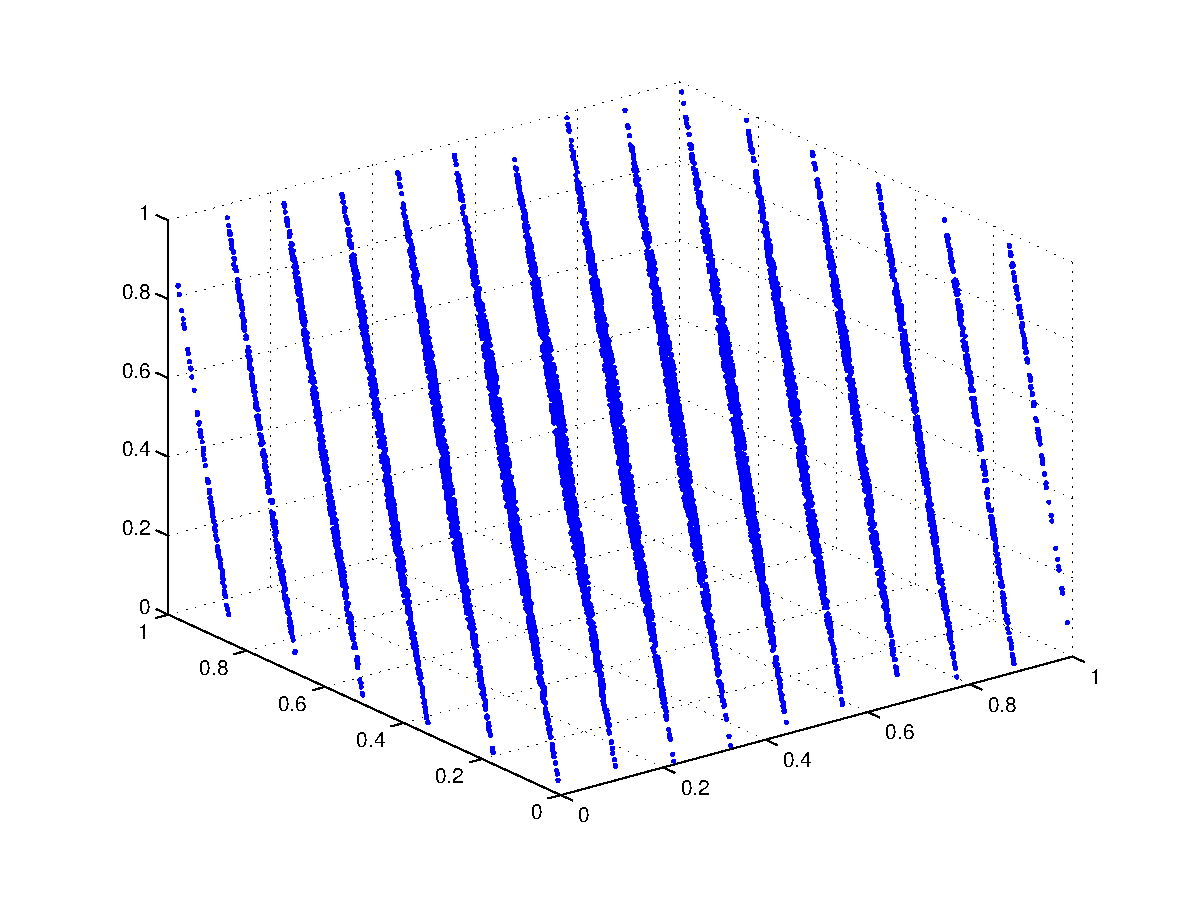
\includegraphics[width=8cm]{images/ibm_randu.eps}
	\caption{Verteilung aufeinanderfolgender Zufallszahlen des IBM Randu Algorithmus}
	\label{fig:IBMRandu}
\end{figure}


\subsubsection{Die rand() Funktion von C}
Durch die einfache und sehr effiziente Berechnung finden LCG Generatoren viel Verbreitung in der Praxis. So verwendet die C-Funktion \texttt{rand()} nach dem LCG-Algorithmus mit den Konstanten $a=1103515245$, $c=12345$, $m=2^{31}$, und dem mit der Funktion \texttt{srand()} gesetzten Startwert. \cite{rng:randFunction} Eine gängige Praxis ist es, den Startwert mit der aktuellen Systemzeit zu initialisieren. Ein entsprechendes Code-Snippet liegt im Github-Repository bei. \cite{rng:githubRepo} \\

\newpage
\subsection{Lehmer Generator} \label{subsec:Lehmer}
Der Lehmer-Generator ist eine Unterart der LCG Generatoren, nach folgender Rekursionsvorschrift:

\begin{equation}
	x_{i+1} = a x_{i} \mod{m}
	\label{equ:lehmer}
\end{equation}

wobei $m$ eine Primzahl sein muss. Sie zeichnen sich gegenüber Standard LCG Generatoren durch eine höhere Periodendauer aus. David W. Hutchinson in seinem Paper \textit{``A new uniform pseudorandom number generator''} 1966 \cite{rng:Hutchinson1966} vor, das Modul  $m = 2^{31} - 1 = 2'147'483'647$ zu wählen. Damit ist der Generator in 32-bit Systemen relativ effizient umsetzbar. Eine optimale Wahl des Parameters $a$ blieb er jedoch schuldig. \\

Erst Jahre später, im Oktober 1988, publizierten Stephen K. Park und Keith W. Miller im Journal \textit{Communications of the ACM}\footnote{ACM: Association for Computing Machinery: Renommierte wissenschaftliche Gesellschaft zur Förderung der Informatik} einen Artikel \cite{rng:ParkMiller1988}, in welchem Sie genauer auf eine gute Wahl von $a$ eingingen. Sie zeigten sich in ihrem Paper \textit{`` Random number generators: good ones are hard to find.''} sehr besorgt über die gängige Praxis von Zufallsgeneratoren - insbesondere auch in Fach- und Lehrbüchern:

\begin{quote}
	\textit{Many generators have been written, most of them have demonstrably non-random characteristics, and some are embarrassingly bad.}
\end{quote}
\begin{flushright}
	- Stephen Park, Keith Miller, 1988 \cite{rng:ParkMiller1988}
\end{flushright}

Sie kritisieren insbesondere, dass, wie am Beispiel IBM gezeigt, häufig mehr Fokus auf Codeoptimierung anstatt auf die Qualität der Generatoren gelegt wird. Neben der klaren Aussage, dass das Modul $m$ unbedingt eine Primzahl sein soll, stellen Sie folgende Anforderungen an die Wahl des Faktoren $a$:

\begin{enumerate}
	\item Die Funktion $f(z) = a z \mod m$ erzeugt die maximal mögliche Periode $m$.
	\item Die komplette erzeugte Sequenz ist zufällig.
	\item $f(z)$ kann effizient auf einem 32-bit System implementiert werden.
\end{enumerate}

Aus Bedingung 3. folgt, dass die von Hutchinson \cite{rng:Hutchinson1966} vorgeschlagene Wahl von $m = 2^{31} - 1$ fast optimal für 32-bit Systeme ist. Aus den mehr als 2 Milliarden möglichen $a$ erfüllen nur einzelne alle drei Bedingungen. Bereits 1969 schlugen Lewis, Goodman, Miller \cite{rng:LewisGoodmanMiller1969} die Wahl von $a = 7^5 = 16'807$ vor, bis zum Paper von Park und Miller fand dies aber kaum Beachtung. Genau diese Kombination wurde von Park und Miller als \textbf{Minmal Standard}  für Random Number Generators bezeichnet. In der Literatur wird für diesen RNG häufig die Bezeichnung Park-Miller RNG benutzt. \\

In den 90er Jahren wurde der Park-Miller Generator von einigen Seiten kritisiert, sodass diese offiziell als neue Faktoren $a = 48271$ oder $a = 69621$ empfahlen und ausdrücklich darauf hinwiesen dass der Algorithmus nur als Minimal Standard zu verstehen ist. So hat sich dieser auch weiterhin als Standard in vielen Bibliotheken etabliert und ist eindeutig als schneller, einfacher, aber trotzdem qualitativ hochwertiger RNG zu empfehlen.

\newpage
\subsubsection{Implementation des Minimal Standard}
Eine logisch erscheinende Implementation in C sieht wie folgt aus:
\begin{lstlisting}[style=C]
	double random(int* seed) {
		const int a = 16807;
		const int m = 2147483647;
		
		*seed = (a * (*seed)) % m;
		return ((double)*seed) / m;
	}
\end{lstlisting}
wobei die Variable \texttt{seed} den aktuellen Integer Wert speichert, und die Funktion \texttt{random} einen \texttt{double}-Wert zwischen $0$ und $1$ zurückgibt. Auf den meisten Systemen wird diese Variante \textbf{nicht} funktionieren. Der maximale Wert der Multiplikation \texttt{a * (*seed)} beträgt $16807*2147483646 \approx 1.03 * 2^{45}$, was deutlich grösser als ein Integer ist. Um solche Fehler zu verhindern schlagen Park und Miller vor, jede Implementation zu prüfen indem mit $x_1 = 1$ der Wert $x_{10001} = 1043618065$ verifiziert wird. \\

Eine Möglichkeit, solche Fehler zu umgehen liegt in der Verwendung von Floating-Point Zahlen. Dabei ist anzumerken ist, dass der Modulo-Operator für Floating-Point in C nicht definiert ist, sondern die Funktion \texttt{fmod()} aus dem \texttt{math.h} Header verwendet werden muss. Trotzdem muss darauf geachtet werden, dass die Mantisse mindestens 46-bit oder grösser ist, d.h. es muss bereits der \texttt{double}-Datentyp\footnote{double: 52-bit Mantisse} anstelle von \texttt{float}\footnote{float: 23-bit Mantisse} verwendet werden. \\

Der deutlich elegantere Ansatz ist es, jegliche Werte kleiner als $2^{32}$ zu halten. Dazu wird $m$ geschrieben als

\begin{equation}
	m = aq + r
\end{equation}
mit 
\begin{equation}
	q = \lfloor m/a \rfloor \qquad \text{und} \qquad r = m \text{ mod } a
\end{equation}
Daraus ergibt sich: (Beweis, siehe \cite{rng:ParkMiller1988})
\begin{equation}
	a x \text{ mod } m = 
		\begin{cases}
			a \left(x \text{ mod } q\right) - r \lfloor x / q\rfloor & \text{wenn }\geq 0 \\
			a \left(x \text{ mod } q\right) - r \lfloor x / q\rfloor + m & \text{sonst}
		\end{cases}
\end{equation}
Damit ergeben sich Zwischenresultate bis $2^{32}$, womit eine einfache Implementation möglich ist:

\begin{lstlisting}[style=C]
	double random(int* seed) {
		const int a = 16807;
		const int m = 2147483647;
		const int q = 127773;
		const int r = 2836;
		
		int k = *seed / q;
		*seed = a * (*seed - k*q) - k*r;
		if(*seed < 0)   *seed += m;
		return (double)*seed / m;
	}
\end{lstlisting}
Diese Implementation ist nicht nur sehr schnell, sondern verfügt, wie von Park und Miller \cite{rng:ParkMiller1988} nachgewiesen, über sehr gute Eigenschaften um als Minimal Standard verwendet zu werden.

\newpage
\subsection{Mersenne-Twister} \label{subsec:MersenneTwister}
Der Mersenne-Twister Algorithmus zeichnet sich durch eine extrem hohe Periode von $2^{19937}-1 \approx 4.3 \cdot 10^{6001}$ aus. Die Periodenlänge ist eine Mersenne-Primzahl\footnote{Mersenne-Primzahl: Primzahl der Form $2^{n}-1$} und gibt dem Algorithmus den Namen. Die Ausgabesequenz ist bis zur Dimension 623 gleichverteilt, d.h. werden die ausgegebenen Zahlen als Vektoren bis Dimension 623 interpretiert, so sind diese Vektoren immer gleichverteilt. \\

Der Mersenne-Twister Algorithmus arbeitet mit 624 Zustandswörtern $Y_1 \dots Y_N$ von typischerweise 32-bit Länge. Diese Zustände werden zu Beginn des Algorithmus initialisiert. Dies wird häufig mit dem in Abschnitt \ref{subsec:RandomDev} beschriebenen Random-Device oder mit einfacheren Zufallszahlgeneratoren wie dem LCG gemacht. Je besser (d.h. zufälliger) die Initialisierung, desto früher sind die generierten Zahlen auch zufällig. Ist dies nicht gewährleistet, kann $Y[2]$ mit einem zufälligen Seed, z.B. der Uhrzeit, initialisiert werden und $800'000$ Zahlen generiert werden, bevor der Algorithmus benutzt wird. So ist eine gute Gleichverteilung sichergestellt. \\

Der Algorithmus für alle darauf folgenden Zufallszahlen $Y_i$ für $i>N$ werden wie folgt berechnet:

\begin{align}
	h &:=  Y_{i-N} - Y_{i-N} \mod{2^{31}} + Y_{i-N+1} \mod{2^{31}} \\
	Y_i &:= Y_{i-227} \oplus \left\lfloor \frac{h}{2} \right\rfloor \oplus \left( \left(h \mod{2} \right) \cdot 9908b0df_{\text{hex}}\right)
\end{align}

Um sicherzustellen, dass alle 32-bit gleichverteilt sind, werden die Zufallszahlen $Z$ aus $Y$ wie folgt berechnet: 
\begin{align}
	x &:= Y_{i} \oplus \left\lfloor \frac{Y_i}{2^{11}} \right\rfloor \\
	y &:= x \oplus \left(\left(x \cdot 2^7\right) \wedge 9d2c5680_{\text{hex}} \right) \\
	z &:= y \oplus \left(\left(y \cdot 2^{15}\right) \wedge efc60000_{\text{hex}} \right) \\
	Z_i &:= z \oplus \left\lfloor \frac{z}{2^{18}} \right\rfloor
\end{align}

Obwohl der Mersenne-Twister Algorithmus sehr kompliziert scheint, ist die Ausführung relativ schnell. Zusammen mit den bereits beschriebenen Vorteilen hat dies dazu geführt, dass der Mersenne-Twister der Standard-Zufallszahlengenerator in vielen Bibliotheken, wie z.B. der \textit{GNU Scientific Library} ist.


\newpage
\section{Tests von RNGs}

Die Probleme beim Testen eines Zufallszahlengenerators können an folgendem Beispiel visualisiert werden: Angenommen, ein RNG soll Zufallszahlen mit Mittelwert $\mu = 7$ generieren. Wenn als erster Wert $6.5$ ausgegeben wird, ist das in Ordnung. Wenn jetzt aber als nächster Wert $7.5$ erzeugt wird, um den Mittelwert $\mu = 7$ zu erreichen, würde das den Generator vorhersehbar machen. Der Mittelwert wird nie genau $7$ betragen, sollte aber bei längeren Sequenzen in der Nähe von $7$ liegen \cite{rng:BeautifulTesting}. Diese Ungenauigkeiten verdeutlichen, dass jedes Testverfahren für RNGs gelegentlich fehlschlagen wird. Ein Test der immer erfüllt wird, deutet darauf hin dass der Ausgang des RNG zu vorhersehbar ist. \\


\newpage
\printbibliography[heading=subbibliography]
\end{refsection}

\section{Integration}

Die Monte-Carlo-Methode kann zur nummerischen Bestimmung von Integralen benutzt werden. Dazu werden in dem Definitionsbereich der Integrandenfunktion Zufallsereignisse generiert, deren Gesamtheit das Integral bestimmt. Im einzelnen können dazu die Methoden herangezogen werden, die im vorigen Abschnitt zu Erzeugung von Ereignissen benutzt wurden. Für die Bestimmung eines Integrals ist es wichtig, mit welcher Methode am effektivsten eine gewünschte Genauigkeit erreicht werden kann.
% TODO HIT or Miss, etc...?

\newpage

\section{Beispiel $\pi$}

Zur Illustration wird die Zahl $\pi$ mittels Monte Carlo Integration angenähert. Um die Komplexität möglichst gering zu halten, wird das Hit or Miss Verfahren angewendet.
Ein Kreis mit Radius r hat eine Grundfläche von $\pi r^{2}$. Ein Einfaches Integrationsvolumen $\Omega^{2}$ für den Kreis ist ein Quadrat mit Seitenlänge $2 r$ und somit einer Grundfläche von $4 r^2$.

\begin{figure}[h]
	\centering
	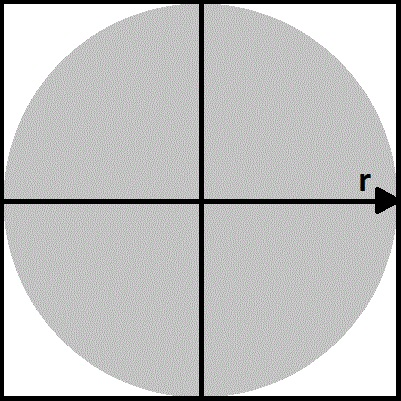
\includegraphics{images/Kreis_ganz.jpg}
	\caption{Kreis im Integrationsvolumen  $4 r^{2}$}
	\label{fig:GanzerKreis}
\end{figure}
Wird der Nullpunkt des Koordinatensystemes im Ursprung des Kreises angenommen, kann das Problem offensichtlich auf den ersten Quadranten reduziert werden, ohne die Flächenverhältnisse zu verändern. Die neuen Flächen werden nun zu $\dfrac{1}{4}\pi r^{2}$ für den Kreis und $r^{2}$ für $\Omega^{2}$.

\begin{figure}[h]
	\centering
	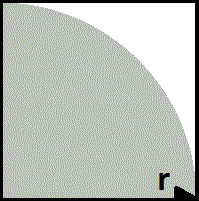
\includegraphics{images/Kreis_viertel.jpg}
	\caption{Ein viertel des Kreises im Integrationsvolumen $r^{2}$}
	\label{fig:ViertelrKreis}
\end{figure}
Werden nun die Fläche des Integrationsraumes mit der des Viertelkreises verglichen, resultieren die Wahrscheinlichkeiten, ob ein HIT or Miss Ereignis im Kreis (grau) oder ausserhalb liegt. Wird der Radius $r = 1$ gesetzt, entsprechen die Flächen gerade der Wahrscheinlichkeit. Die Abfrage, ob ein Hit vorliegt, ist bei dem Viertelkreis einfach. Ist die Entfernung des Ereignis kleiner als $r$ zum Ursprung, handelt es sich um ein Hit. Die Entfernung kann mit dem Pythagoras ausgerechnet werden.

\begin{equation}
	P_{in} = \frac{\pi}{4}
\end{equation}

\begin{equation}
	P_{out} = 1-\frac{\pi}{4}
\end{equation}

\begin{equation}
	Hit, wenn x^{2} + y^{2} < 1
\end{equation}
Um als Ergebnis der Simulation die Zahl $\pi$ angenähert zu erhalten, müssen die Hits(k) mit der Anzahl generierter MC Ereignissen(N) dividiert werden und mit 4 Multipliziert werden.
\begin{equation}
	\pi \approx \dfrac{4 k}{N}
\end{equation}

\end{document}